\documentclass[margin,line]{resume}
\usepackage[T1]{fontenc}
\usepackage{lmodern}
\usepackage[hidelinks]{hyperref}
\usepackage{tikz}
\setlength{\textheight}{9.7in}

\begin{document}
\begin{tikzpicture}
\clip (0,0) circle (1cm) ;
\node[anchor=center] at (0,0) {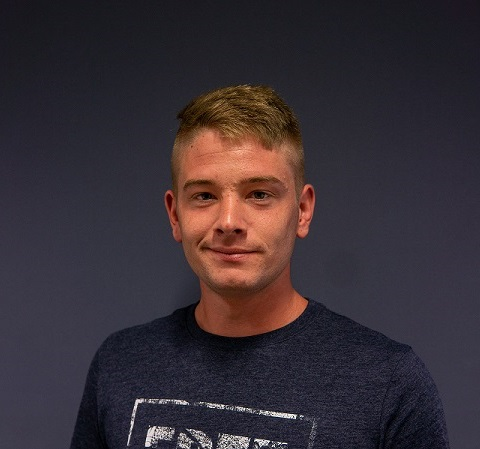
\includegraphics[width=2cm]{assets/myface}};
\end{tikzpicture} \name{\Large Andrea Hrelja}
\begin{resume}

    \section{\mysidestyle Contact\\Information}

    Email: \href{mailto:andhrelja@hotmail.com}{\texttt{andhrelja@hotmail.com}} \hfill
    GitHub: \href{https://github.com/andhrelja}{\texttt{github/andhrelja}} \hfill
    LinkedIn: \href{https://www.linkedin.com/in/andhrelja/}{\texttt{linkedin/andhrelja}} \hfill

    \vspace{3mm}

    \section{\mysidestyle About Me}

    IT enthusiast coming from Istra county in Croatia. During my 4 years of professional experience as a Data Engineer, I have worked with various production systems and clients, as a team member and as a one-man band. I am a positive, detail-oriented, productive individual with a can-do attitude, ready to start working on that new project.

    \vspace{3mm}

    \section{\mysidestyle Professional\\Experience}

        \textbf{Cloud Infrastructure}, Kern AI \vspace{2mm}\\\vspace{1mm}%
    \textsl{Cloud Engineer} \hfill \textbf{11/2023 -- Present}\\
    Migrate Digital Ocean deployed production system to Azure Kubernetes Service

    \begin{itemize}
        \item Designed a system migration plan (on-prem and Digital Ocean to Azure Kubernetes Service) with the team
		\item Developed a CI/CD pipeline using OpenTofu, GitHub Actions and Kubernetes
		\item Consolidated environment-specific infrastructure stacks into a single OpenTofu stack, orchestrated by GitHub Actions
		
    \end{itemize}

    SDLC: Strategy, Design, Development, Testing, Maintenance

    \textbf{Banking Industry}, iOLAP \vspace{2mm}\\\vspace{1mm}%
    \textsl{DataOps Engineer} \hfill \textbf{12/2021 -- 11/2023}\\
    Build a CI/CD system to streamline DW development on Snowflake for multiple teams in the organization

    \begin{itemize}
        \item Developed a version controlled SQL CI/CD solution designed by a System Architect using Python, AWS and Snowflake technologies (CodeBuild, GitHub (Actions), Flyway, custom Python packages)
		\item A colleague DevOps Engineer and I developed the CI/CD from scratch, collaborating with the client and the solution users (multiple SQL development teams) in a "Startup" fashion
		\item Directly communicated with the client and was involved in business decisions (discovery, requirements, strategy)
		
    \end{itemize}

    SDLC: Strategy, Design, Development, Testing, Maintenance

    \textbf{Hospitality Industry}, iOLAP \vspace{2mm}\\\vspace{1mm}%
    \textsl{Data Engineer} \hfill \textbf{07/2021 -- 10/2021}\\
    Build a Data Warehouse (ELT + DW)

    \begin{itemize}
        \item Developed an ETL solution designed by a System Architect using Python and AWS technologies (DynamoDB, Glue, Lake Formation, Lambda, Redshift, dbt)
		\item Collaborated with the System Architect to design the system and a DevOps Engineer to design the AWS infrastructure
		\item Not included in business decisions or client communication, my focus was delivering a reliable ELT system
		
    \end{itemize}

    SDLC: Design, Development, Testing

    \textbf{Oil \& Gas Industry}, iOLAP \vspace{2mm}\\\vspace{1mm}%
    \textsl{BI Developer} \hfill \textbf{03/2020 -- 06/2021}\\
    Support and Enhance an existing infrastructure

    \begin{itemize}
        \item Collaborated on supporting and enhanceing enterprise ETL solutions using Oracle and other technologies (Oracle ODI, Oracle WebLogic, Tibco Data Virtualization, Spotfire BI)
		\item Working with an enterprise production system and a well-structured Azure Boards, I transitioned into a Mid Data Engineer
		\item Included in analyses that impact business decisions, mostly in the discovery phases where I would elaborate effects of proposed solutions to the client
		
    \end{itemize}

    SDLC: Design, Development, Testing, Maintenance

    \textbf{Banking Industry}, iOLAP \vspace{2mm}\\\vspace{1mm}%
    \textsl{SQL Developer} \hfill \textbf{08/2019 -- 02/2020}\\
    Build a Data Warehouse (DW only)

    \begin{itemize}
        \item Collaborated on a DW development using pure SQL on on-prem servers
		\item Created automated Python tests
		\item Not included in business decisions or client communication
		
    \end{itemize}

    SDLC: Development, Testing


    \vspace{3mm}
    
    \section{\mysidestyle Published\\Works}

    \textbf{Prediction of COVID-19 tweeting: classification based on graph neural networks}, M. Petrović, A. Hrelja, A. Meštrović, DOI: 10.23919/MIPRO55190.2022.9803426


    \vspace{3mm}

    \section{\mysidestyle Programming\\Experience}

    \emph{Languages:} Python, SQL (any), Bash, JavaScript, \LaTeX \\
    \emph{Other Technologies:} Oracle, AWS, Snowflake, GitHub Actions, Django, dbt, Flyway...

    \vspace{3mm}

    \section{\mysidestyle Education}

    \textbf{Faculty of Informatics and Digital Technologies, University of Rijeka} \vspace{2mm}\\\vspace{1mm}%
    \textsl{Master's degree, Computer Engineering} \hfill \textbf{10/2020 -- 12/2022}\\
    Master's thesis: \href{{https://zir.nsk.hr/islandora/object/infri%3A999}}{{\texttt{{Information Spread Analysis on Twitter}}}}


    \vspace{3mm}
    
        \section{\mysidestyle Languages}

    Croatian: First language (L1) \\
	English: C1 \\
	Italian: A2 \\

\end{resume}
\end{document}